\section{Compatibility with the exact Stokes transport}
\label{sec:Stokes}

The factor $e^{-Au/4}$ in the positive-action boundary amplitude has an
independent analytic interpretation. It is the finite change in the
exponential $e^{-A/t}$ when the inverse coordinate changes from $q$ to
$t=qe^{-V}$. We make that statement precise using the exact forward
completion already established in the incoming report.

\subsection{The exact forward input and the sign convention}

For positive $t$ define the exact remainder
\begin{equation}\label{eq:R-exact}
 R_{\mathrm{ex}}(t)
 =\F(t)-\frac12\{\log(1/t)+\gamma\}^2-C_*.
\end{equation}
It includes the linear term $-t/4$ and has the formal expansion $R(t)$.
This convention differs from the predecessor's calligraphic
$\mathcal R_0$, which begins at degree two. The two lateral sums of our
entire formal remainder satisfy
\begin{equation}\label{eq:exact-lateral-input}
 R_\pm(t)=R_{\mathrm{ex}}(t)\pm\frac12J(t),\qquad
 J(t)=4\pi\ii\sum_{m\ge1}d(m)E_1(Am/t),
\end{equation}
where
\[
 E_1(x)=\int_x^\infty \frac{e^{-v}}v\dd v,\qquad x>0.
\]
The exact identification of the arithmetic mean with
\eqref{eq:R-exact} is the Mellin--Voronoi completion theorem of
\cite[Section 5]{incoming}; it is an imported analytic identity.
The sign of its jump also follows directly from
\eqref{eq:R-Borel-lattice}: upper continuation of the first logarithm
past a positive branch point gives imaginary part $-\pi$. Thus
upper minus lower continuation of $\widehat R$ is positive $4\pi\ii/\xi$
times the accumulated divisor weight, and its Laplace transform is
$J(t)$.

The series for $J$ converges normally for $\re(1/t)>0$. For $t\to0^+$,
\begin{align}
 J(t)&=\frac{4\pi\ii}{A}\,t e^{-A/t}\{1+O(t)\},
       \label{eq:J-leading}\\
 J'(t)&=\frac{4\pi\ii}{t}\sum_{m\ge1}d(m)e^{-Am/t}.
       \label{eq:J-derivative}
\end{align}
The first formula follows by one integration by parts in $E_1$, with
the terms $m\ge2$ exponentially smaller. Termwise differentiation proves
the second. These formulas also hold with uniform bounds in the small
complex neighborhoods used below.

\subsection{Uniform transport in the slow parameter}

\begin{proposition}[Leading inverse jump with its shifted amplitude]
\label{prop:Stokes-transport}
Fix $U>0$. For all sufficiently small real $q>0$, uniformly for
$0<u\le U$, let $V_\eta$ be the small solution of
\begin{equation}\label{eq:eta-inverse}
 V_\eta+\frac u2V_\eta^2
 +uR_{\mathrm{ex}}(qe^{-V_\eta})
 +\frac{\eta u}{2}J(qe^{-V_\eta})=0,\qquad \eta\in\{0,1,-1\}.
\end{equation}
Put $t_0=qe^{-V_0}$ and
\[
 D=1+uV_0-ut_0R_{\mathrm{ex}}'(t_0).
\]
Then
\begin{align}
 V_+-V_-&=-\frac{uJ(t_0)}{D}
                  +O_U\bigl(u^2q e^{-2A/q}\bigr),
                  \label{eq:jump-linear-transport}\\
 &=-\frac{4\pi\ii}{A}\,u q
       \exp\{-A/q-Au/4\}\{1+O_U(q)\}.
                  \label{eq:jump-q-transport}
\end{align}
Consequently, under the physical specialization \eqref{eq:physical},
the lateral inverses $t_\pm=qe^{-V_\pm}$ satisfy
\begin{equation}\label{eq:physical-jump}
 t_+-t_-=\frac{\ii}{\pi}\frac{q^2}{X}
       \exp\left\{-\frac Aq-\frac{A}{4X}\right\}
       \{1+O(q)\},\qquad X\to+\infty.
\end{equation}
\end{proposition}
\begin{proof}
The finite Mellin expansion, with differentiation on a smaller sector,
gives
\[
 R_{\mathrm{ex}}(t)=-t/4+O(t^2),\quad
 R_{\mathrm{ex}}'(t)=-1/4+O(t),\quad
 R_{\mathrm{ex}}''(t)=O(1).
\]
For example the differentiated bounds follow either by shifting
\eqref{eq:mellin} farther before differentiating, or by Cauchy's estimate
applied to the finite-order remainder. They are uniform near the
positive ray. A contraction on $|v|\le M_Uu q$ therefore gives the
solution at $\eta=0$ and
\begin{equation}\label{eq:small-exact-inverse}
 V_0=uq/4+O_U(uq^2),\qquad D=1+O_U(q).
\end{equation}
The derivative of the fixed-point map is $O_U(q)$ on this disk.
The exponentially small added term in \eqref{eq:eta-inverse} preserves
the contraction for $|\eta|\le1$ and gives
\[
 \delta_\eta:=V_\eta-V_0=O_U(uq e^{-A/q}).
\]

Here are bounds sufficient to retain the square of the exponential in
the remainder. In a complex disk $|v-V_0|\le c_0q$, with $c_0$ fixed,
\[
 \left|\exp\{-A e^v/q\}\right|\le C_U e^{-A/q}.
\]
Indeed $V_0=O_U(q)$ and $e^v-1=O_U(q)$. The divisor series and
\eqref{eq:J-derivative} then give
\[
 |J(qe^{-v})|\le C_Uq e^{-A/q},\qquad
 |\partial_v J(qe^{-v})|\le C_Ue^{-A/q}.
\]
The second derivative of
$v+uv^2/2+uR_{\mathrm{ex}}(qe^{-v})$ is $O_U(u)$.
Taylor expansion at $V_0$ in \eqref{eq:eta-inverse} consequently yields
\[
 D\delta_\eta+\frac{\eta u}{2}J(t_0)
 =O_U\!\left(u|\delta_\eta|^2+
                    u e^{-A/q}|\delta_\eta|\right)
 =O_U\bigl(u^2q e^{-2A/q}\bigr).
\]
Subtracting the equations for $\eta=1$ and $-1$ proves
\eqref{eq:jump-linear-transport}. The bounds retain all displayed
powers of $u$, so they are uniform down to $u=0$.

Finally \eqref{eq:small-exact-inverse} gives
\[
 t_0=q\{1-uq/4+O_U(uq^2)\},\qquad
 \frac A{t_0}=\frac Aq+\frac{Au}{4}+O_U(q).
\]
Insert these relations and \eqref{eq:J-leading} into
\eqref{eq:jump-linear-transport} to obtain
\eqref{eq:jump-q-transport}. The Taylor expansion of $qe^{-v}$ gives
$t_+-t_-=-t_0(V_+-V_-)$ to the same relative accuracy.
Since $4\pi/A=1/\pi$ and $u=1/X$, this proves
\eqref{eq:physical-jump}.
\end{proof}

The positive Borel logarithm in \eqref{eq:B0-model} has coefficient
$2u e^{-Au/4}/\xi$. Its upper-minus-lower logarithmic discontinuity has
the sign $-2\pi\ii$, consistent with \eqref{eq:jump-q-transport}.
This is a consistency check between two proved calculations. We have
not inferred a complete Stokes discontinuity from a merely continuous
boundary remainder. Nor do we identify an arithmetic mean after nonlinear
inversion with a nonlinear median summation operation. The exact inverse
transport in \cite[Section 8]{incoming} already distinguishes those
operations.

\section{Reproducible verification and numerical behavior}
\label{sec:verification}

The proofs establish the infinite statements. The accompanying program
checks exact finite identities, evaluates complete finite coefficient
formulas, and tests the scale of the asymptotic errors. It does not use
the proposed asymptotic formulas to generate the coefficients being
compared.

\subsection{Exact checks}

The script \texttt{verification/verify.py} constructs the polynomials
$C_1,\ldots,C_{12}$ over $\Q[u]$ by two independent routes:
coefficient recursion in the implicit equation and the finite Lagrange
formula \eqref{eq:C-finite}. It then substitutes the result back into
\eqref{eq:implicit} through degree twelve. It checks the sign, valuation,
degree, Catalan top coefficient, and the exact lowest-coefficient
identities of Proposition~\ref{prop:structure}.

The same run checks the rational factorial inequalities through $n=100$.
For the gamma ratio it checks the rational consequence
$n^{k-1}b_{n-k+1}/b_n\le k3^k$ for every $1\le k\le n$, including
$k=n$; the sharper $ke^k$ bound is proved analytically in
Lemma~\ref{lem:factorial}. Convolution powers are checked through $n=32$. Exact symbolic
algebra checks the first-correction sums. In total, the executed run
passed \textbf{5,890 exact assertions}. The JSON record separates those
assertions by category; \texttt{coefficients\_exact.txt} contains the
complete degree-twelve coefficient list.

\subsection{Complete finite sums and independent precision checks}

Direct factorials become very large. The numerical implementation
therefore normalizes the convolution recurrence by its endpoint gamma
factor before forming \eqref{eq:D-formula}. The main table evaluates
\emph{every} finite summand $1\le k\le n$: there is no mathematical
truncation in these coefficient values.

The recorded grid contains 70 cases, with
\[
 n\in\{64,65,128,129,256,257,512,513,1024,1025\},
\]
and the seven parameter choices
$u=0.01,0.05,0.1,0.2,0.5$, $u=0.1+0.05\ii$, and
$u=1/\log(n+e)$. The last choice exercises a parameter tending to zero.
The main arithmetic uses a 64-bit-significand extended-range
\texttt{longdouble}, whose properties are recorded and checked at
runtime. A platform that aliases this type to ordinary binary64 is
rejected explicitly.

An independent 80-decimal-digit \texttt{mpmath} calculation at the
recorded cross-check indices agrees with the main calculation to within
$2.36\times10^{-19}$ in the program's relative-or-absolute normalization.
Evaluation of the exact coefficient polynomials agrees with the
high-precision route to within $4.68\times10^{-81}$.
A separate binary64 convolution computation at larger indices differs
by at most $3.12\times10^{-16}$. That secondary check truncates at
$k=256$; its omitted contribution to $D_n/(4b_n)$ is bounded by the
exact rational certificate recorded in \texttt{results.json}, whose
value is less than $2.861\times10^{-18}$ for $|u|\le1/2$.
This certificate bounds omitted terms, not floating-point roundoff.
The main table needs no such truncation certificate.

For the table and plots define
\[
 Z_n=\frac{(-1)^{n+1}A^nC_n}{4ub_n},\qquad
 E_0=\left|\frac{Z_n-H_\epsilon}{H_\epsilon}\right|,\qquad
 E_1=\left|\frac{Z_n-H_\epsilon-K_\epsilon/n}{H_\epsilon}\right|,
 \quad \epsilon=n\bmod2,
\]
where $H_\epsilon=H_\epsilon(cu)$.
Table~\ref{tab:errors} gives representative errors at $u=0.1$.
The normalization is the leading amplitude $H_\epsilon$, not the
computed coefficient. Figure~\ref{fig:errors} shows both parities and
the scaled second-order residual.

\begin{table}[htbp]
\centering
\caption{Leading-amplitude-normalized errors for even coefficients at
$u=0.1$. Every finite Lagrange summand is included.}
\label{tab:errors}
\begin{tabular}{rcc}
\toprule
$n$ & Leading amplitude only: $E_0$ & With the $1/n$ correction: $E_1$\\
\midrule
64   & $4.52796\times10^{-2}$ & $3.96799\times10^{-3}$\\
128  & $2.15988\times10^{-2}$ & $9.42970\times10^{-4}$\\
256  & $1.05580\times10^{-2}$ & $2.30119\times10^{-4}$\\
512  & $5.22080\times10^{-3}$ & $5.68550\times10^{-5}$\\
1024 & $2.59610\times10^{-3}$ & $1.41311\times10^{-5}$\\
\bottomrule
\end{tabular}
\end{table}

\begin{figure}[htbp]
\centering
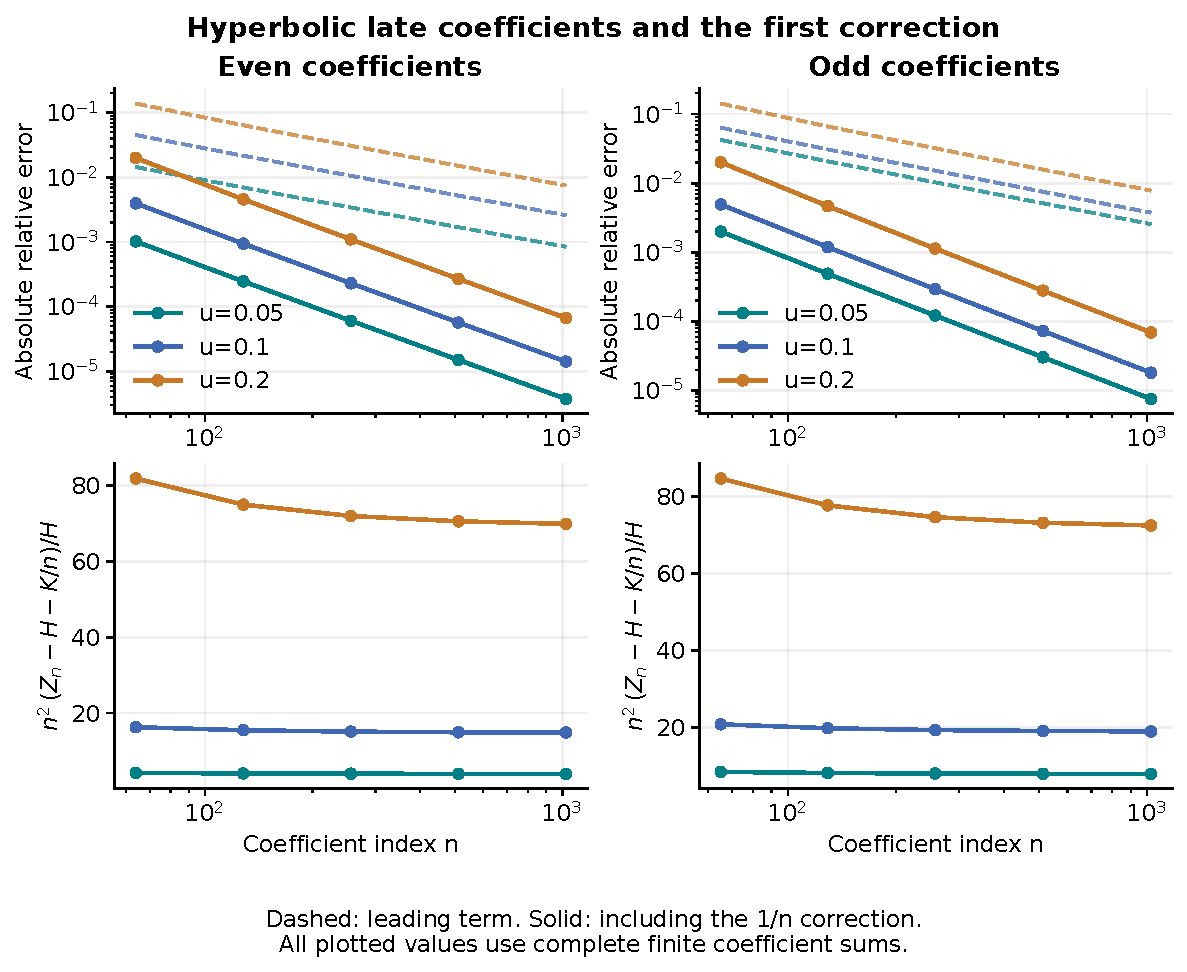
\includegraphics[width=\textwidth]{verification/asymptotic_errors.pdf}
\caption{Executed finite-sum diagnostics from the supplied program.
The observed first- and second-order decay agrees with the proved
uniform expansion. The plot is evidence of implementation consistency,
not a proof of an asymptotic estimate.}
\label{fig:errors}
\end{figure}

At the largest even and odd indices, the first correction reduces the
observed errors by factors between 37 and 592 over the tested parameters.
The recorded software versions, precision checks, full CSV, and
machine-readable results make this comparison reproducible. No interval
certification of the floating-point output is claimed.

\FloatBarrier
\section{Source audit and proposed repository integration}
\label{sec:audit}

\subsection{The inspected snapshot and the limits of the audit}

All repository references in this contribution are pinned to commit
\begin{center}
\texttt{8f5afd4d7565df808359f6a0c22f87f79a119bb9}
\end{center}
dated 12 October 2026. The research used the Polylogarithms and
Transseries indexes, relevant source chapters, and the three incoming
research archives listed below. The package's \texttt{provenance.json}
records exact paths and cryptographic hashes.

\begin{enumerate}
 \item \texttt{Resonant\_Lambert\_Inverse\_Transseries\_2026-10-12.zip}:
 the principal predecessor, including its inverse-coefficient theorem,
 exact completion and Stokes transport, and explicit research questions.
 \item \texttt{ProveIt\_Lambert\_Polylog\_Order\_Jets\_2026-10-12.zip}:
 order derivatives, resonant jets, and the arithmetic Lambert interface.
 \item \texttt{ProveIt\_Quadratic\_Polylog\_Boundaries\_2026-10-12.zip}:
 the quadratic feedback problem and its boundary regimes.
\end{enumerate}

The related integrated chapters are
\nolinkurl{01-resonant-jets.tex}, \nolinkurl{01-lambert-moments.tex}, and
\nolinkurl{01-quadratic-feedback.tex} under the Polylogarithms manuscript.
The related Transseries reports include
\nolinkurl{Polylogarithm_Resonance_And_Inverse_Transseries},
\nolinkurl{Quadratic_Polylogarithm_Feedback_Boundary_Completion}, and
\nolinkurl{Resonant_Polylogarithm_Transseries}.
In particular, the last report already proves an arbitrary-order
Fermi--Dirac Borel completion. We do not present that existing result
as a new contribution.

No specific false theorem was established in this scoped audit.
The unproved hyperbolic amplitudes are explicitly labelled conjectural
in their source; its coarser coefficient bound is valid for the purpose
there. Resolving that conjecture is an addition to the source, not a
retroactive claim that its proof was incorrect. This audit does not
certify every file in either research program.

\subsection{Concrete updates supported by the present proofs}

The following integration changes are justified without expanding the
claims beyond what is proved.

\begin{enumerate}
 \item \textbf{Promote the two amplitude conjectures.}
 In Section 11.1 of the principal predecessor, replace the conjectural
 status of \texttt{eq:conj-even} and \texttt{eq:conj-odd} by a reference
 to Theorem~\ref{thm:main}. State uniformity on $0<u\le U$ and preserve
 the distinction between coefficient index and physical target size.
 The first correction can be added as a separate strengthening.

 \item \textbf{Sharpen the inverse Borel conclusion.}
 The source's radius argument is strengthened by
 Theorem~\ref{thm:Borel-models}: both nearest real actions are genuine
 singularities for every fixed complex $u\ne0$. Include the explicit
 logarithmic and logarithmic--dilogarithmic models, with their stated
 boundary regularity.

 \item \textbf{Resolve the continuation part of Section 11.2.}
 Cite Theorem~\ref{thm:inverse-continuation} and the original closure
 theorem of Sauzin. Formulate the allowed set as $A\Z$, including the
 possibility of a singular origin on another sheet. Leave the exact
 active lattice and full local or alien description as research questions.

 \item \textbf{Retain the formal and analytic distinctions.}
 A zero-radius sector series is not made convergent by inserting
 $u=1/X$. The sectorial inverse is provided by summation as in
 Theorem~\ref{thm:inverse-summability}. Also retain the explicit
 $-t/4$ term when translating the source's degree-two remainder to the
 convention of this article; omitting it removes the amplitude shift.
\end{enumerate}

The accompanying \texttt{INTEGRATION.md} gives suggested destination
paths, stable theorem labels, and reviewable replacement prose. It
proposes a new report directory under \nolinkurl{Analysis/Transseries}
and a cross-reference from Polylogarithms. No existing source file is
silently replaced, and this package does not contain a repository push.

\section{Further research questions}
\label{sec:research}

The proofs isolate several concrete next steps. We separate problems
that appear approachable by extending the present coefficient argument
from those requiring additional analytic machinery.

\subsection{All inverse-index orders and higher boundary regularity}

Can one prove, for each fixed $N$, a locally uniform expansion
\[
 \frac{(-1)^{n+1}A^nC_n(u)}{4ub_n}
 =\sum_{j=0}^{N-1}\frac{K_{\epsilon,j}(u)}{n^j}
                  +O_{U,N}(n^{-N}),\qquad \epsilon=n\bmod2,
\]
with $K_{\epsilon,0}=H_\epsilon(cu)$ and
$K_{\epsilon,1}=K_\epsilon(u)$?
The expected route is to retain all configurations with a fixed small
total excess away from the large index, expand the gamma ratios and
$T_{n,k}$ to the same order, and bound the remainder uniformly before
summing over $k$. An explicit recursion for the resulting polynomial
coefficients multiplying $\cosh(cu)$ and $\sinh(cu)$ would be more useful
than isolated higher-order formulas.

Such a theorem would produce Borel models built from
$\Li_1,\ldots,\Li_N$, where $\Li_1(w)=-\log(1-w)$, with a
$C^{N-1}$ remainder on the closed disk. More precisely, keeping the
terms $j=0,\ldots,N-1$ above leaves Borel coefficients
$O(A^{-n}n^{-N-1})$, whose derivatives through order $N-1$ converge
absolutely on the boundary. Smooth boundary control of every finite
order would still not, by itself, identify a complete local analytic
singularity type.

\subsection{A paired-action factorial calculus}

The finite-phase theorem proves the leading transformation law
\[
 \kappa_\omega\longmapsto
 \kappa_\omega e^{\lambda_\omega\rho u},\qquad
 \lambda_\omega=A/\omega.
\]
Can the factorial asymptotic calculus of \cite{Borinsky2018} be extended
in a form that handles several equal-modulus actions and cancellations
uniformly in a parameter? For the present model one seeks simultaneous
coefficient expansions in
$\Gamma(n-1-j)A^{-(n-1-j)}$ and
$\Gamma(n-1-j)(-A)^{-(n-1-j)}$, with a rigorously justified
composition rule.
That result should reproduce Theorem~\ref{thm:main} and explain which
finite forward coefficients control each successive order. It would
also apply to root-of-unity twists and character-weighted Lambert sums.

\subsection{Which arithmetic lattice points are active?}

Theorem~\ref{thm:inverse-continuation} confines possible singularities to
$A\Z$, and Theorem~\ref{thm:Borel-models} proves activity at $\pm A$.
Determine the singular behavior at $\pm2A,\pm3A,\ldots$ on specified
continuation paths. At $2A$, for example, the forward divisor weight
$d(2)$ can interact with two nonlinear contributions of action $A$.
The problem is to separate these sources without double counting and
to decide whether any cancellations occur for special $u$.
A precise result should specify the sheet, path convention, and local
coordinate at every action.

\subsection{The full local singularity and Stokes operator}

The continuous and continuously differentiable boundary remainders do
not determine a complete analytic singularity type. Can one show that
the primitive-action singularities admit a logarithm times a convergent
or explicitly resurgent germ, and compute that germ to all orders?
The exact analytic transport in Section~\ref{sec:Stokes} gives a strong
constraint but is not a substitute for a local Borel theorem.
Care is needed at the origin on other sheets: differentiation in the
coordinate-inversion proof can change the order of a pole. A global
claim of \emph{simple resurgence} needs a separate proof.

\subsection{A growing slow parameter and a new saddle regime}

The present bounds are uniform on every fixed disk in $u$, with no
lower bound. They are not uniform as $|u|\to\infty$.
The leading exponential sum favors $k$ of size approximately $|cu|$.
When $u=u_n$ grows with $n$, both the gamma-ratio correction
$k^2/n$ and the feedback correction $uk^2/n$ can become significant.
Identify the largest growing ranges that still admit relative
hyperbolic asymptotics, and determine the transition law when the
feedback correction is order one. The size of the relative correction
$K_\epsilon(u)/(nH_\epsilon(cu))$
suggests a positive-real transition near $u$ of order $n^{1/3}$;
this is a scaling heuristic, not a theorem.

\subsection{Optimal truncation for the physical inverse}

For fixed $u$, the ratio of successive coefficient magnitudes suggests
optimal sector truncation near $n=A/|q|$, modulo the parity amplitudes.
The physical problem couples $q=e^{\gamma-X}$ and $u=1/X$, placing
that truncation order far beyond polynomial size in $X$.
Can one obtain a sharp remainder for the real inverse after optimal
truncation, together with a terminant description of the lateral jump?
The uniform coefficient theorem supplies necessary late-term data;
such a remainder theorem also needs analytic estimates on the summed
inverse and its Stokes neighborhoods.

\subsection{Moving away from exact resonance}

The incoming work contains parameter jets at exact polylogarithmic
resonance. Extend the present result to nonzero order displacement
$\varepsilon$, with coefficient bounds uniform as
$\varepsilon\log(1/q)$ changes size. The coalescing-pole core depends on
this combined variable, and its order jets contain logarithms; the
regular forward coefficients also vary with $\varepsilon$. In the
source's normalization, for $n\ge2$ and $\varepsilon$ near zero,
\[
 r_n(\varepsilon)=
 \frac{2\{1+(-1)^n\cos(\pi\varepsilon)\}}{A^n n!}
 \Gamma(n-\varepsilon)\Gamma(n+\varepsilon)
 \zeta(n-\varepsilon)\zeta(n+\varepsilon).
\]
Thus an odd regular tail is already activated away from resonance, as
proved in \cite{incoming}. The new target is a uniform theorem for the
late \emph{inverse} coefficients, specifying when this mechanism and
nonlinear odd-sector production reinforce or cancel one another, with
the corresponding action amplitudes.

\subsection{Exact verification and reusable formal components}

The finite coefficient formula, valuation identities, and the
reciprocal-binomial convolution bounds are natural candidates for
proof-assistant formalization. They involve finite algebra and
inequalities before any analytic continuation is introduced.
A separate numerical project could replace the diagnostic arithmetic
by interval bounds for selected large-index coefficients and for the
sectorial inverse. Neither task should be confused with the other:
finite exact computations check an implementation, whereas a
formalized uniform convolution theorem would certify the step that
turns all finite coefficients into an asymptotic result.
